% Emacs, this is -*-latex-*-
\title{\href{http://www.libpng.org/pub/png}{PNG (Portable
  Network Graphics)}}

\maketitle
\tableofcontents

\section{What is PNG?}
\href{https://www.youtube.com/watch?v=EFUYNoFRHQI}{PNG}\footnote{Notice
that only the first part of the video describes PNG. The second part
refers to QOI that is a different image compression scheme.} is an
open (free of patents) raster-graphics file format,
\href{https://en.wikipedia.org/wiki/Portable_Network_Graphics}{developed
  by the W3C}, that supports lossless image
compression~\cite{roelofs1999png}. PNG exploits the intra-channel
\href{https://en.wikipedia.org/wiki/Image_compression}{spatial} and
\href{https://en.wikipedia.org/wiki/Data_compression}{statistical
  redudancy} (no \href{https://en.wikipedia.org/wiki/YUV}{color
  transform} is used).

\section{\href{http://www.libpng.org/pub/png/book/}{Posibilities}}
\begin{itemize}
\item \href{https://en.wikipedia.org/wiki/Lossless_compression}{Fully
  lossless}.
\item Only
  \href{https://en.wikipedia.org/wiki/Raster_graphics}{raster} (not
  \href{https://en.wikipedia.org/wiki/Vector_graphics}{vectorized})
  images.
\item Better funtionality and performance than
  \href{https://en.wikipedia.org/wiki/GIF}{GIF (Graphics Interchange
    Format)}, that uses an patented implementation of the
  \mylink{LZW}{LZW} algorithm, and
  \href{https://en.wikipedia.org/wiki/TIFF}{TIFF (Tagged Image File
    Format)}.
\item Free usage and free from patents.
\item
  \href{https://en.wikipedia.org/wiki/Palette_(computing)}{Palletized
    images} (up to 256 colors), true color images (up to
  48-bits/pixel) and grayscale images (up to 16-bits/pixel).
\item On-the-fly encoding and decoding (streamability).
\item \href{https://en.wikipedia.org/wiki/Alpha_compositing}{Alpha
  channels} (variable transparency).
\item \href{https://en.wikipedia.org/wiki/Gamma_correction}{Gamma
  correction} (cross-platform control of image brightness).
\item
  \href{https://en.wikipedia.org/wiki/Progressive_scan}{Progressive}
  and
  \href{https://en.wikipedia.org/wiki/Interlacing_(bitmaps)}{interlazed}
  images.
\item
  \href{http://www.libpng.org/pub/png/book/chapter08.html#png.ch08.div.6}{Progressive
    reconstructions} by means of spatial scalability.
\end{itemize} 

\section{The PNG codec}

PNG is based on
\href{https://en.wikipedia.org/wiki/Differential_pulse-code_modulation}{DPCM}
(filtering in the PNG nomenclature) and the
\href{https://en.wikipedia.org/wiki/DEFLATE}{DEFLATE}, which is a text
compressor based on
(\href{https://en.wikipedia.org/wiki/Huffman_coding}{Huffman coding}
and
\href{https://en.wikipedia.org/wiki/LZ77_and_LZ78}{LZ77})~\cite{nelson96datacompression}. All
these ``text'' compressors are completely reversible.

\begin{figure}
  \centering
  %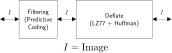
\includegraphics[width=20cm]{PNG_codec_ext}
  \svgfig{graphics/PNG_codec}{6cm}{600}
  \caption{Architecture of the PNG codec. ${\mathbf I}$ represents the
    RGB image,and ${\mathbf E}$ the prediction error resulting of the
    predictive coding. As it can be seen, DEFLATE does not modify
    ${\mathbf E}$, but only finds a more compact representation of the
    same information.}
\end{figure}

Notice that DEFLATE is applied indepently to each channel. For
example, in the case of a RGBA image, four independent DEFLATE
code-streams are generated.

\section{Filtering (predictive encoding)}
\begin{itemize}
\item Optional step.
\item
  \href{https://en.wikipedia.org/wiki/Differential_pulse-code_modulation}{DPCM
    (Differential Pulse Code Modulation)} stage that reduces the
  spatial correlation.
\item Pixels are translated to prediction residues (errors):
  \begin{equation*}
    {\mathbf E} = {\mathbf I} - \hat{\mathbf I}
  \end{equation*}
  where $\hat{\mathbf I}$ is an image prediction.
\item The entropy of the residue image is typically smaller than in
  the original image, and the residues follow a
  \href{https://en.wikipedia.org/wiki/Laplace_distribution}{Lapace
    probability distribution}, centered in 0 (the average of the
  prediction error is 0).
\item Available predictors (``filters''):
  \begin{center}
    \begin{tabular}{c}
      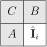
\includegraphics[width=3cm]{contexto_prediccion} \\
      \begin{tabular}{rcl}
        Type & Predictor & Prediction \\
        \hline
        0 &	None 	& $\hat{\mathbf I}_i\leftarrow 0$ \\
        1 &	Sub 	& $\hat{\mathbf I}_i\leftarrow A$ \\
        2 &	Up 	& $\hat{\mathbf I}_i\leftarrow B$ \\
        3 &	Average & $\hat{\mathbf I}_i\leftarrow (A+B)/2$ \\
        4 &	Paeth 	& $\hat{\mathbf I}_i\leftarrow A + B - C$
      \end{tabular}
    \end{tabular}
  \end{center}
\item To increase the compression ratio (considering that the best
  predictor can depend on the area of the image that is being
  compressed), the predictor can be changed (and pbviously this is
  signaled) in the ``middle'' of the encoding of an image.
\end{itemize}

\section{``Deflate'' (encoding)}
\begin{itemize}
\item It's a generic text-compression algorithm based on
  \mylink{LZ77}{LZ77} and \mylink{Huffman_coding}{Huffman coding},
  written by
  \href{https://en.wikipedia.org/wiki/Jean-loup_Gailly}{Jean-loup
    Gailly} and \href{https://en.wikipedia.org/wiki/Mark_Adler}{Mark
    Adler}\footnote{Authors of The Data Compression Book
    \cite{nelson96datacompression}}.
\item LZ77 removes the statistical \mylink{redundancy}{redundancy} of
  high order (remember that the preditor has removed the spatial
  redundancy).
\item The Huffman encoder removes the statistical redundancy of order
  0. The \mylink{probabilistic_models}{probabilistic model} used is
  adaptive and initially empty.
\item The amount of redundancy removed depends on several factors
  (such as the configuration of the DEFLATE parameters and the
  information stored in the image) resulting in an unpredictable
  output bit-rate.
\end{itemize}

\section{Entropy and lossless compression}
To estimate the
\href{https://en.wikipedia.org/wiki/Redundancy_(information_theory)}{redundancy}
we have basically two options:
\begin{enumerate}
\item Compute the
  \href{https://en.wikipedia.org/wiki/Entropy_(information_theory)}{0-order
    (memoryless source) entropy} of the signal: the higher the
  entropy, the lower the redudancy. In fact, if we suppose that the
  samples of the signal are uncorrelated, the 0-order entropy is an
  exact measure of the expected bit-rate achieved by an
  \href{https://en.wikipedia.org/wiki/Arithmetic_coding}{arithmetic
    encoder} (the most efficient entropy compressor). Unfortunately,
  the 0-order entropy is usually only a estimation of the redundancy,
  i.e., lower bit-rates can be achieved in practice after using a high-order
  decorrelation.
\item A better way is to use an
  \href{https://en.wikipedia.org/wiki/Data_compression}{lossless
    compressor}: the higher the length of the compressed file compared
  to the length of the original file, the lower the
  redundancy.\footnote{If the length of the compressed file is equal or
  larger than the length of the original file, then, for the compressor
  that we are using, there is not redundancy in the original
  representation.} Notice, however, that although this estimation is
  more accurate than the 0-order entropy, in general, it depends on the
  compressor (different algoritms can provide different
  estimations).
\end{enumerate}

\begin{comment}
\section*{Let's go to the lab!}
\begin{itemize}
\item Fill-up the following table:
  \begin{tabular}{r|llll|l}
    \hline
    & \multicolumn{4}{c}{Image}     & \\
    \hline
    Codec & \href{http://www.hpca.ual.es/~vruiz/images/lena.png}{lena} & \href{http://www.hpca.ual.es/~vruiz/images/boats.png}{boats} & \href{http://www.hpca.ual.es/~vruiz/images/peppers.png}{pepers} & \href{http://www.hpca.ual.es/~vruiz/images/zelda.png}{zelda} & Average \href{https://en.wikipedia.org/wiki/Data_compression_ratio}{Compression Ratio} \\
    \hline
    \href{https://imagemagick.org/script/convert.php}{convert} & & & & & \\ 
    \hline
  \end{tabular}
\end{itemize}
\end{comment}

\section{Resources}

\renewcommand{\addcontentsline}[3]{}% Remove functionality of \addcontentsline
\bibliography{image-compression, text-compression}
